\documentclass[
%% TIKZ_CLASSOPTION %%
tikz
]{standalone}
\usepackage{amsmath}
\usetikzlibrary{matrix}
%% EXTRA_TIKZ_PREAMBLE_CODE %%
\begin{document}
%% TIKZ_CODE %%
  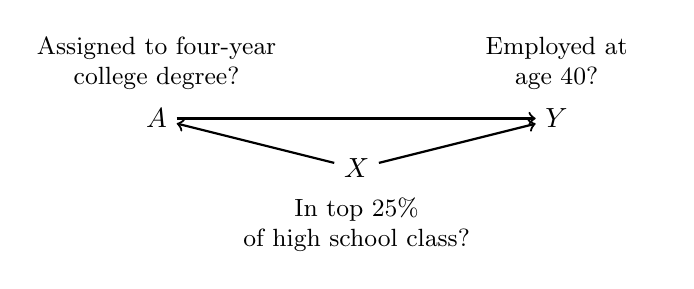
\begin{tikzpicture}[x = .5in, y = .25in]
    \node at (-3,0) {};
    \node at (3,0) {};
    \node (x) at (0,-1) {$X$};
    \node (a) at (-2,0) {$A$};
    \node (y) at (2,0) {$Y$};
    \draw[->, thick] (x) -- (a);
    \draw[->, thick] (a) -- (y);
    \draw[->, thick] (x) -- (y);
    % Labels
    \node[anchor = north, font = \small, align = center] at (x.south) {In top 25\%\\of high school class?};
    \node[anchor = south, font = \small, align = center] at (a.north) {Assigned to four-year\\college degree?};
    \node[anchor = south, font = \small, align = center] at (y.north) {Employed at\\age 40?};
  \end{tikzpicture}
\end{document}
